\documentclass[nonatbib,numbers,10pt]{sigplanconf}

% Code listing
%\usepackage{minted}
%\usemintedstyle{tango}
\usepackage{amsmath}
\usepackage{amssymb}
\usepackage{epigraph}
% Colors
\usepackage{xcolor}
\colorlet{CodeBg}{gray!90}
\usepackage{color, colortbl}
\definecolor{Gray}{rgb}{0.9,0.9,0.9}
% Graphs
\usepackage{tikz}
\usetikzlibrary{calc}
\usetikzlibrary{trees}
\usetikzlibrary{positioning}

\newcommand\todo[1]{\textcolor{red}{#1}}

\title{$D^3$ as a MCFL}

\authorinfo{Orestis Melkonian, Konstantinos Kogkalidis}{Utrecht University, The Netherlands}{o.melkonian@uu.nl, konstantinos@riseup.net}

\begin{document}
\toappear{}

\maketitle

\begin{abstract}
Aspernatur fugit autem numquam corporis repellendus quasi. Et nisi veritatis consequatur adipisci iure. Sint quos aspernatur ea iste est. 
\end{abstract}

%\ccsdesc[500]{Software and its engineering~Program verification}
%\ccsdesc[500]{Theory of computation~Program semantics}

%\keywords{Predicate transformer semantics; Weakest Liberal Pre-condition (WLP); Guarded Command Language (GCL); Hoare logic; automated testing; formal verification}

\epigraph{As you set out for Ithaka\\
hope the voyage is a long one,\\
full of adventure, full of discovery.}{\textit{C. P. Cavafy\\ Ithaka}}

\section{Introduction}
Our goal with this paper is the analysis of the 3-dimensional Dyck Language, $D^3$ under the scope of a 2-multiple context-free language, 2-MCFL. In this chapter, we start by providing some concise definitions and a brief overview of interesting correspondences and properties of the $D^3$. The goal of this chapter is to simply introduce the reader to some possibly less known concepts rather than to fully extend upon them. For a deeper and more detailed view of the ideas presented, we direct the interested reader towards our list of references, which provide significantly more information.
\subsection{Definitions}
\paragraph{MIX}
Borrowing notation from \todo{Kazanawa}, we define the $MIX_d$ language as the language over a d-symbol, lexigraphically ordered alphabet $a_1 < a_2 < ... a_d$, whose words $w$ satisfy the condition:
\begin{itemize}
\item[(D1)]  $ \# a_i(w) = \# a_j(w) \ \forall \ i,j \in d $
\end{itemize}
where $ \#x(w)$ refers to the number of occurrences of symbol $x$ within word $w$.
\paragraph{Dyck Language}
We use $D^n$ to refer to the Dyck language over the same alphabet. $D^d$ is defined as a subset of $MIX_d$, whose words $w$ abide to one additional constraint:
\begin{itemize}
\item[(D2)] For every prefix $v$ of $w$, $ \#a_i(v) \geq \#a_j(v) \ \forall i, j \ \in d$ such that $i < j$.
\end{itemize}

The $D^2$ language corresponds to the language of well-bracketed parentheses, and $D^d$ generalizes this over an arbitrarily large alphabet.
\paragraph{MCFL}
Multiple context free languages, abbreviated MCFLs, is the class of languages generated by multiple context free grammars, abbreviated MCFGs. Multiple context-free grammars are a mildly context-sensitive grammar formalism that, rather than strings, operate on tuples of strings. MCFGs contain partial functions defined as the concatenation of constant strings from the terminal alphabet and components of their arguments \todo{̈Gotzmann}. An m-multiple context-free grammar, m-MCFG, acts upon tuples of at most m-elements. The language generated by an m-MCFG is an m-MCFL. The class of MCFLs is interesting to the domain of linguistics, because it is believed to capture the intricacies of natural languages. 

\subsection{Correspondences}
%
\paragraph{Young Tableaux}
A standard Young Tableau is defined as an assortment of $n$ boxes into a ragged (or jagged, ie. non-rectangular) matrix containing the integers $1$ through $n$ and arranged in such a way that the entries are strictly increasing over the rows (from left to right) and columns (from top to bottom). Reading off the entries of the boxes, one may obtain the \textit{Yamanouchi} word $w_Y =w_1 w_2 ... w_n$ with $w_i$ corresponding to symbol $a_j$, where j is the row containing entry $i$.\\
\todo{Example}\\
In the case of $D^d$, the Tableau associated with these words is in fact \textit{rectangular} of size $n \times d$, and the length of the corresponding word (called a \textit{balanced or dominant Yamanouchi word} in this context) is $dn$, where $n$ is the number of occurrences of each unique symbol and $d$ the total number of unique symbols \todo{Moortgat}.
Practically, the rectangular shape ensures constraint (D1), while the ascending order of elements over rows and columns ensures constraint (D2). In that sense, a rectangular standard Young tableu of size $n \times 3$ is, as a construct, an alternative way of uniquely representing the different words of $D^3$. We present two examples below:\\
\begin{table}[h!]
  \centering
    \begin{tabular}{| l | c | r |}
    \hline
    1 & 2 & 3 \\
    \hline
    4 & 5 & 6 \\
    \hline
    7 & 8 & 9 \\
    \hline
    \end{tabular}
  \caption{A simple table}
\end{table}

\paragraph{Promotions and Orbits}
Having presented the concept of a Young Tableau, we can now move ahead with the \textit{Jeu-de-taquin} algorithm. When operating on a rectangular Table $T(n,d)$, Jeu-de-taquin consists of the following steps:
\begin{table}[h!]
\begin{enumerate}
\item[(1)] Reduce all elements of T by 1 and replace the first utem of the first row with an empty box $ \Box (x,y) := (1,1)$. 
\item[(2)] While the empty box is not at the bottom right corner of T, $ \boxdot(x,y) \neq (n,d)$, do:
\begin{enumerate}
\item[(a)] Pick the minimum of the elements directly to the right and below the empty box, and swap the empty box with it. $ T(x, y) := min(T_{(x+1,y)}, T_{(x,y+1)})$, $ \Box (x',y') = (x+1, y)$ (in the case of a right-swap) or $\Box (x',y') = (x,y+1)$ (in the case of a down-swap).
\end{enumerate}
\item[(3)] Replace the empty box with $dn$.
\end{enumerate}
\caption{Jeu-de-taquin algorithm for rectangular Tableux}
\end{table}

The table obtained through Jeu-de-taquin on T is called its promotion $p(T)$. $k$ successive applications of Jeu-de-taquin result in $p^k(T)$. \todo{M. Haiman} shows that there exists a $m$ such that $p^m(T)=T$. In other words, the promotion defines an equivalence class, which we name an \textit{orbit}, which cycles back to itself. Orbits dissect the space of $D^d_n$ into disjoint sets, ie. there is no word $w$ whose Tableu $T_w$ belongs to more or less than a single orbit. 
\paragraph{Constrained Walk}
A Dyck word can also be visualized as a constrained \textit{walk} within the first quadrant of $\mathbb{Z}^2$. We can assign each alphabet symbol $x$ a vector value $\vec{v_x} \in \mathbb{Z}^2$ such that all pairs of $(\vec{v_i},\ \vec{v_j})$ are linearly independent and:
\begin{equation*}
\vec{v_a} + \vec{v_b} + \vec{v_c} = \vec{0}
\end{equation*}
One such value assignment could for instance be:
\begin{table}[h!]
\[\begin{array}{c c}
Symbol & Vector\\
\hline
a & (\ 1\ ,\ 0\ )\\
b & (-1,\ 1\ )\\
c & (\ 0\ ,-1)\\
\end{array}\]
\caption{Symbols as vectors}
\end{table}

We can then picture Dyck words as routes starting from $(0,0)$. (D1) means that each route must also end at $(0,0)$, while (D2) means that the $x$ and $y$ axes may never be crossed. An example walk follows:
\begin{figure}[h!]
    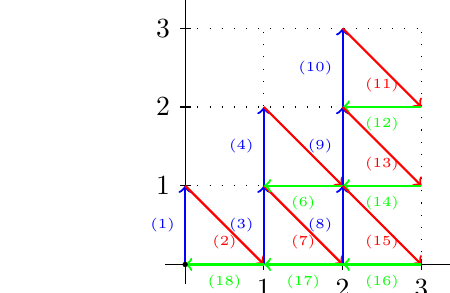
\begin{tikzpicture}[scale=1]
    \draw[loosely dotted] (0,0) grid (3,3);
    \path[use as bounding box] (-2,1) rectangle (3,3);
    \draw[->] (-0.25,0) -- (3.5,0) node[right] {$x$};
    \draw[->] (0,-0.25) -- (.,3.5) node[left] {$y$};
    \foreach \x/\xtext in {1/1, 2/2, 3/3}
    \draw[shift={(\x,0)}] (0pt,2pt) -- (0pt,-2pt) node[below] {$\xtext$};
    \foreach \y/\ytext in {1/1, 2/2, 3/3}
    \draw[shift={(0,\y)}] (2pt,0pt) -- (-2pt,0pt) node[left] {$\ytext$};
    \draw [blue, ->, thick] (0,0) -- node[left] {\tiny{(1)}} (0,1);
    \draw [red, ->, thick] (0,1) -- node[below] {\tiny{(2)}} (1,0);
    \draw [blue, ->, thick] (1,0) -- node[left] {\tiny{(3)}} (1,1);
    \draw [blue, ->, thick] (1,1) -- node[left] {\tiny{(4)}} (1,2);
	\draw [red, ->, thick] (1,2) -- (2,1);
	%\draw [green, ->, thick] (2,1) -- (1,1);
	\draw [red, ->, thick] (1,1) -- node[below] {\tiny{(7)}} (2,0);
	\draw [blue, ->, thick] (2,0) -- node[left] {\tiny{(8)}} (2,1);
    \draw [blue, ->, thick] (2,1) -- node[left] {\tiny{(9)}} (2,2);
    \draw [blue, ->, thick] (2,2) -- node[left] {\tiny{(10)}} (2,3);
    \draw [red, ->, thick] (2,3) -- node[below] {\tiny{(11)}}(3,2);
	\draw [green, ->, thick] (3,2) -- node[below] {\tiny{(12)}} (2,2);
	\draw [red, ->, thick] (2,2) -- node[below] {\tiny{(13)}} (3,1);
	\draw [green, ->, thick] (3,1) -- node[below] {\tiny{(14)}} (2,1);
	%\draw [red, ->, thick] (2,1) -- node[below] {\tiny{(5)}} (1,2);
	\draw [green, ->, thick] (2,1) -- node[below] {\tiny{(6)}} (1,1);
    \draw [red, ->, thick] (2,1) -- node[below] {\tiny{(15)}} (3,0);
	\draw [green, ->, thick] (3,0) -- node[below] {\tiny{(16)}} (2,0);
	\draw [green, ->, thick] (2,0) -- node[below] {\tiny{(17)}} (1,0);
	\draw [green, ->, thick] (1,0) -- node[below] {\tiny{(18)}} (0,0);
    \draw[fill=orange,color=black] circle (0.75pt);
    \end{tikzpicture}
\\
\caption{The constrained walk of \textit{abaabcbaaabcbcbccc}}
\end{figure}
\paragraph{$A_2$ Combinatorial Spider Webs}
The $A_2$ \textit{irreducible combinatorial spider web} is a category which \todo{Khu} defines as a planar directed graph $D$, with no multiple edges embedded in a disk that satisfies conditions W1 through W3:
\begin{enumerate}
\item[(W1)] $D$ consists of positive and negative edges, with each edge being oriented from one of the negative edges to one of the positive edges. 
\item[(W2)] All boundary vertices have degree $1$ while all internal vertices have degree $3$.
\item[(W3)] $D$ is non-elliptic, ie. all internal faces of $D$ have at least $6$ faces.
\end{enumerate}

$A_2$ is a way of constructing visually intriguing, minimal parses of $D^3$ words. To make this clear, we first define the three \textit{positive} and three \textit{negative} edges which assume the role of states in the parsing process of $D^3$, aligned with their corresponding alphabet symbols (or sequence thereof):
\begin{table}[h!]
\[\begin{array}{c c}
$State$ & $Symbol Sequence$\\
\hline
A^{+} & a\\
B^{+} & b\\
C^{+} & c\\
A^{-} & bc\\
B^{-} & ac\\
C^{-} & bc\\
\end{array}\]
\caption{Edges of the $A_2$ growth algorithm}
\end{table}

We now present a version of \todo{Petersen's} summation of the \textit{growth algorithm} in web form, which models the various possible interactions of edges-states, rephrased to our problem's scope.

\todo{Growth Rules}


The edges on the upper level can be seen as input nodes which, interacting with one another, produce either one or a pair of output edges. The soundness of each individual \textit{growth rule} is immediately obvious. On a higher level, what the growth algorithm achieves is to:
\begin{enumerate}
\item[(a)] Merge two neighbouring edges of the same polarity into one of the opposite, and propagate it downwards.
\item[(b)] Perform the closures of $\{A+$, $A-\}$ and $\{C-$, $C+\}$.
\item[(c)] Swap the horizontal position of pairs of states between which no immediate interaction exists, such that either of them eventually ends up neighbouring another edge with which it can be eliminated.\footnote{This property is referred to as crossing removal. \todo{Petersen} shows that the outcome of crossing removal is uniquely determined and independent of the order of removal.}
\end{enumerate}

At termination, the growth algorithm produces an $A_2$ web with no \textit{dangling strands} and no edge crossing \todo{Petersen}. 
\subsection{Properties}
\paragraph{Cardinality}
The number of words produced by $D^3_n$, $| \! | D^3_n | \! |$, corresponds to the A005789 integer sequence\footnote{Refer to the Online Encyclopedia of Integer Sequences (\textit{OEIS})} [\todo{Moortgat}].
Interestingly, the number of orbits $| \! | O(D) | \! |$ exhibits symmetricity between the alphabet size $d$ and the number of occurrences $n$, ie. $| \! | O(D^n_d) | \! | = | \! | O(D^d_n) | \! |$.
\begin{table}[h!]
\begin{center}
\begin{tabular}{c | c c c c c }
$d \backslash n$ & 2 & 3 & 4 & 5 & 6\\
\hline
2 & 2 & 5 & 14 & 42 & 132\\
\rowcolor{Gray}
\ & 1 & 2 & 3 & 6 & 14\\
3 & 5 & 42 & 462 & 6006 & 87516\\
\rowcolor{Gray}
\ & 2 & 6 & 44 & 406 & 4896\\
\end{tabular}
\end{center}
\caption{Word and orbit (grayscale) cardinality of $D^d_n$}
\end{table}
\paragraph{Non-wellnestedness}
The property of well-nestedness can be informally described as the absence of rules that permute the tuples of interacting states in such a way that their corresponding dependency trees interleave \todo{Joshi 1997}. A more formal definition is given by \todo{Salvati, MIX}, which we will not include. In the case of $D^3$, there seem to exist cross-serial dependencies, violating the above constraint, and rendering $D^3$ non-wellnested.

\section{Modeling}
Having established the necessary vocabulary, we can now begin tackling the elusive problem of parsing $D^3$ via a 2-MCFG. This chapter's contents follow a chronological order, tracking our progressively larger, more complex and more abstract grammars.
\subsection{Triple Insertion}
During our early days of initiation to the world of $D^3$, the problem seemed only as a natural continuation to (much simpler) ones we had encountered before. With its difficulty not immediately apparent, our first modeling attempt was rather naive. Yet despite its naivety, it is still a relevant component of the grammars to follow, so we present it here.

The grammar of \textit{triple insertion}, as its name suggests, simply inserts in order the three alphabet symbols \textit{a, b} and \textit{c} in any way possible given a non-terminal state $W$ (for \textit{word}) consisting of the tuple $(x,y)$. This non-terminal produces a variety of tuples that respect both (D1) and (D2). The end-word is produced through the concatenation of $(x,y)$ as produced by a single-arity state $S(xy)$.

\todo{Grammar}

\todo{Counter-Example}
Despite its compact size (and inarguable naivety), our first grammar is nevertheless relatively expressive. The prominent weak point is its inability to manage the effect of \textit{straddling}, namely the generation of words \todo{that exhibit this characteristic..}.
\subsection{Adding States: Meta-Grammars}
The underwhelming performance of our first attempt signaled for the necessity of more expressive states that would allow for more complex, "longer range" interactions. Intuitively, we imagined a convention by which certain new states would exist. Through controlled interactions, pairs of these new, "incomplete" states could allow parts of words to propagate through the rules until they eventually met their closures or were transformed into a single, new state. In that spirit, we defined the six states of \todo{cross-reference table}. One key difference is that our states may describe strings of arbitrary length, with the polarity now signifying whether the state is carrying an extra character or missing one instead.

In hindsight, we were able to identify a differently represented version of our idea in the growth rules, reaffirming our initial idea that these new states were indeed sound and necessary. The added expressivity, however, came at a cost of rapid rule expansion. Each of the new states could now (potentially) interact with every other, and their means of interaction could become convoluted and hard to decipher or write down. To overcome this obstacle we needed to be able to describe our rules at a slightly more abstract level. For instance, a state $A^{+}(x,y)$ (which now models not just the terminal $a$ but rather an intermediate state for which $ \# b(xy) = \# c(xy) = \# a(xy)-1$), could interact with a $B^{+}(z,w)$ to produce a $C^{-}$ in any of the following ways.
\todo{ways}

Note that for each pair interaction, different constraints pertaining to the order of the permuted concatenated strings need to be preserved, to account for (D2). In the example above, for instance, the internal order of each state's tuple is crucial, but also the external order enforced by the particular pair (ie. the extra $a$ must come before the extra $b$). For that purpose we had to define a method that automatically generates all the allowable permutations, thereby reducing the manual labour required to transcribe and debug rules. 
\todo{define all o}

This additional abstraction, however, is not enough on its own. We still needed the ability to enforce additional constraints related not to the order but rather the positions of concatenated strings. To make this clear, let us present the unique case of $B^{-}$. Unlike other negative states, $B^{-}(x,y)$ has no direct closure unless we actually know it to contain its extra $a$ in the left-side string $x$ and its extra $c$ in $y$. In that case alone can we insert the missing $b$ (obtained from a $B^{+}(z,w)$ between $x$ and $y$. But in order to automatically generate $B^{-}$ states for which this additional condition holds, we need to keep note of the origin of the extra $a$ and $c$, and filter out these rules generated by \todo{all o}. 
\todo{define all c}

The above abstractions significantly accelarated the process of creating and testing grammars, as they allowed us to simply describe rules instead of explicitly defining them. We thus moved from the lowest level of grammars to the higher level of meta-grammars, or grammars of grammars. 

\subsection{Refining States: Rule Inference}



\section{Road to completeness}
Aut saepe voluptatem ipsa. At quae voluptatem quo unde qui a. Commodi omnis quae id doloribus qui et voluptas maxime.

Earum officiis corporis magni provident at vel. Tenetur et hic magni excepturi. Rerum deserunt nesciunt ut at. Illum fuga enim ratione asperiores inventore perferendis est. Consectetur rerum cumque ut eum non omnis voluptatem.

Corrupti nihil voluptatem rem quidem sint. Sunt consequatur laborum voluptas numquam. Nulla libero ut facilis quaerat ullam animi ipsa vitae.

Debitis molestias eos minima omnis est ut. Omnis hic ipsa quam ea modi. Itaque temporibus et earum doloribus aliquid aliquid quod consequatur.

\subsection{First-match policy}
Aspernatur fugit autem numquam corporis repellendus quasi. Et nisi veritatis consequatur adipisci iure. Sint quos aspernatur ea iste est.

Nobis temporibus nihil expedita quia blanditiis. Non voluptatum vel autem voluptatem occaecati libero. Aperiam nostrum id sed voluptatibus fuga. Culpa commodi molestiae molestiae corrupti nam. Sapiente quo commodi architecto exercitationem id ad. Non optio eos perferendis.
\subsection{Growth Rules}
Excepturi eum dolores nisi. Ut non hic quia. Beatae ullam quo est odit adipisci ipsa.

Voluptas consectetur rerum numquam vel qui. Assumenda quas quam nisi quia. Cum cum laborum officia molestiae aspernatur autem. Optio quas recusandae voluptatum eaque eaque. Eligendi cumque maxime ut hic non sequi omnis.

Aperiam et quod minima libero iure. Tenetur harum voluptas earum necessitatibus temporibus optio repudiandae. Magni facilis maiores quisquam error et animi. Modi minima voluptatem et alias. Assumenda et sunt velit. Reprehenderit quod saepe dignissimos qui ab quas.

Provident omnis porro quo quis velit voluptatem. Sunt sit amet dolor. Dolore consequatur est sed maxime molestiae sit iste omnis.

Magni qui commodi quaerat quo velit ut maiores. Non et aspernatur eum quo mollitia rerum. Molestias nam rerum quisquam eveniet dolorem laudantium ex. In adipisci consequatur iusto nisi autem ipsam. Provident aperiam facere sint ut deserunt.

Beatae enim provident quibusdam modi nobis aperiam sunt fugiat. Saepe porro doloribus voluptas qui. Omnis deserunt dolore doloremque tenetur voluptates sit ut.

Voluptas mollitia aut assumenda ut officiis dolores. Et aut debitis animi omnis voluptas aut ipsum. Qui consequuntur iure nesciunt architecto.

Qui et animi molestias. Aperiam optio dolorum et velit non. Eius non occaecati odit autem. Qui saepe et fugiat enim.
\subsection{Meta-grammars}


Aut saepe voluptatem ipsa. At quae voluptatem quo unde qui a. Commodi omnis quae id doloribus qui et voluptas maxime.

Earum officiis corporis magni provident at vel. Tenetur et hic magni excepturi. Rerum deserunt nesciunt ut at. Illum fuga enim ratione asperiores inventore perferendis est. Consectetur rerum cumque ut eum non omnis voluptatem.

Corrupti nihil voluptatem rem quidem sint. Sunt consequatur laborum voluptas numquam. Nulla libero ut facilis quaerat ullam animi ipsa vitae.

Debitis molestias eos minima omnis est ut. Omnis hic ipsa quam ea modi. Itaque temporibus et earum doloribus aliquid aliquid quod consequatur.

Quia maxime qui quas iusto voluptatem sunt placeat officia. Vel natus autem quia magni ex. Labore ipsa aut nihil. Eum cupiditate sint nesciunt.

\subsection{Insights from promotion}
Aut saepe voluptatem ipsa. At quae voluptatem quo unde qui a. Commodi omnis quae id doloribus qui et voluptas maxime.

Earum officiis corporis magni provident at vel. Tenetur et hic magni excepturi. Rerum deserunt nesciunt ut at. Illum fuga enim ratione asperiores inventore perferendis est. Consectetur rerum cumque ut eum non omnis voluptatem.

Corrupti nihil voluptatem rem quidem sint. Sunt consequatur laborum voluptas numquam. Nulla libero ut facilis quaerat ullam animi ipsa vitae.

Debitis molestias eos minima omnis est ut. Omnis hic ipsa quam ea modi. Itaque temporibus et earum doloribus aliquid aliquid quod consequatur.

Quia maxime qui quas iusto voluptatem sunt placeat officia. Vel natus autem quia magni ex. Labore ipsa aut nihil. Eum cupiditate sint nesciunt.

\section{Tooling}
\subsection{}

\section{Results}
\subsection{}
\end{document}
